\documentclass[11pt,a4paper]{scrartcl}
\usepackage[T1]{fontenc}
\usepackage{microtype}
\usepackage{lmodern}
\usepackage{amsmath}
\usepackage{amsfonts}
\usepackage{amssymb}
\usepackage{enumerate}
\usepackage{graphicx}
\usepackage{float}


\def\ojoin{\setbox0=\hbox{$\bowtie$}%
  \rule[-.02ex]{.25em}{.4pt}\llap{\rule[\ht0]{.25em}{.4pt}}}
\def\leftouterjoin{\mathbin{\ojoin\mkern-5.8mu\bowtie}}
\def\rightouterjoin{\mathbin{\bowtie\mkern-5.8mu\ojoin}}
\def\fullouterjoin{\mathbin{\ojoin\mkern-5.8mu\bowtie\mkern-5.8mu\ojoin}}

\begin{document}

\author{Johannes Merkle\\Ralf Vogler}
\title{Query Optimization}
\subtitle{6. Exercise}

\maketitle

\section*{Exercise 1}

We need perform a BFS on the Querygraph to enumerate the relations. We start at $R_0$ resulting in this order:\\
\begin{enumerate}
\item $R_0$
\item $R_3$
\item $R_1$
\item $R_2$
\item $R_4$
\end{enumerate}

\begin{table}[H]
\centering
\begin{tabular}{|l|l|}
\hline
\{5\} &  \\
\{4\} &  \\
\{3\} & \{4\},\{5\} \\
\{3,4\} & \{5\} \\
\{3,5\} & \{4\} \\
\{3,4,5\} & \\
\{2\} & \{4\},\{3,4\},\{3,4,5\} \\
\{2,4\} & \{3\},\{3,5\} \\
\{2,3,4\} & \{5\} \\
\{2,3,4,5\} &  \\
\{1\} & \{3\},\{3,4\},\{3,5\},\{3,4,5\},\{2\},\{2,4\},\{2,3,4\},\{2,3,4,5\} \\
\{1,2\} & \{4\},\{3\},\{3,4\},\{3,5\},\{3,4,5\} \\
\{1,3\} & \{5\},\{4\},\{2\},\{2,4\} \\
\{1,2,3\} & \{5\},\{4\} \\
\{1,2,4\} & \{3\},\{3,5\} \\
\{1,3,4\} & \{5\},\{2\} \\
\{1,3,5\} & \{4\},\{2\},\{2,4\} \\
\{1,2,3,4\} & \{5\} \\
\{1,2,3,5\} & \{4\} \\
\{1,2,3,4,5\} &  \\
\hline
\end{tabular}
\caption{Enumeration of the pairs. The left column shows the results of \textit{EnumerateCsg}, the right column contains the graphs that form a pair with the subgraph in the left column, in the order produced by \textit{EnumerateCmp}. A subgraph is denoted as a set containing the enumeration number.}
\label{tab:dp}
\end{table}

\section*{Exercise 2}

Step 1: compare $((R_0 \Join R_1) \Join R_3)$ to $((R_0 \Join R_3) \Join R_1)$:\\
$C((R_0 \Join R_1) \Join R_3)=2020$, $C((R_0 \Join R_3) \Join R_1)=3000$\\
Remove $R_0 \Join R_3$\\
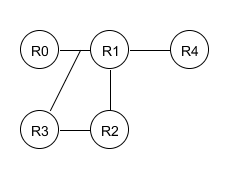
\includegraphics{graph/step1}

Step 2: compare $((R_1 \Join R_2) \Join R_4)$ to $((R_1 \Join R_4) \Join R_2)$:\\
$C((R_1 \Join R_2) \Join R_4)=25100$, $C((R_1 \Join R_4) \Join R_2)=30000$\\
Remove $R_1 \Join R_4$\\
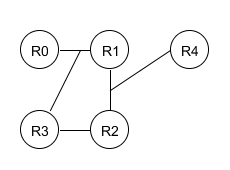
\includegraphics{graph/step2}

\section*{Exercise 3}


\end{document}
